\providecommand{\docroot}{..}
\documentclass[\docroot/reports/draft/report.tex]{subfiles}

\begin{document}

\onlyinsubfile{\tableofcontents}

\subsection{Аналитический вид нечетных мод}

    Для удобства представим базовую нечетную моду в однородном виде и явно выделим множители, зависящие от одной переменной:
    %
    \begin{equation}\label{eq:hl0e}
        (h_{l0}^{(o)})_{ij} = \begin{pmatrix}
            0&0&f^l_{13}(r)u^l_{13}(\theta)\sin\theta\\
            0&0&r f^l_{23}(r)u^l_{23}(\theta)\sin\theta\\
            f^l_{13}(r)u^l_{13}(\theta)\sin\theta &
                r f^l_{23}(r)u^l_{23}(\theta)\sin\theta & 0
        \end{pmatrix} \exp(-i \omega t).
    \end{equation}

    Угловое уравнение \autoref{eq:killeq-hl0} определяет функции $u^l_{13}(\theta)$ и $u^l_{13}(\theta)$:
    %
    \begin{equation*}\begin{aligned}
        u''_{13} + \cot\theta u'_{13} + (l(l+1) - \cosec^2\theta) u_{13} &= 0, \\
        u''_{23} + \cot\theta u'_{23} + (l(l+1) - 4 \cosec^2\theta) u_{23} &= 0,
    \end{aligned}\end{equation*}
    %
    откуда
    %
    \begin{equation}\label{hl0o-u}
        u^l_{13} = P_l^1(\cos\theta), \quad u^l_{23} = P_l^2(\cos\theta),
    \end{equation}
    %
    где $P_l^m$~--- $m$-й присоединенный полином Лежандра первого рода.

    Подстановка метрики в виде \autoref{eq:hl0e} в основное вариационное уравнение в форме \autoref{eq:lagr2var-br-hl0} определит систему дифференциальных уравнений на функции $f^l_{13}(r)$ и $f^l_{23}(r)$:
    %
    \begin{equation*}\begin{gathered}
        (\omega^2 r^2 - L_2) f_{13} + L_2 (r f'_{23} - f_{23}) = 0, \\
        r (\omega^2 f_{23} + f''_{23}) - f'_{13} = 0,
    \end{gathered}\end{equation*}
    %
    где $L_2 = (l-1)(l+2)$. Ее можно привести к виду
    %
    \begin{equation*}\begin{gathered}
        r (r f''_{13} + 2 f'_{13}) - (l(l+1) - \omega^2 r^2) f_{13} = 0, \\
        f_{23} = \frac{2 f_{13} + r f'_{13}}{L_2}.
    \end{gathered}\end{equation*}
    %
    Первое уравнение является уравнением на функции Бесселя полуцелого порядка:
    %
    \begin{equation*}\begin{gathered}
        f^l_{13}(r) = C_1 j_l(\omega r) + C_2 y_l(\omega r), \\
        j_l(r) = \flatfrac{J_{l+1/2}(r)}{\sqrt{r}}, \quad
        y_l(r) = \flatfrac{Y_{l+1/2}(r)}{\sqrt{r}},
    \end{gathered}\end{equation*}
    %
    где $J_l(r)$ и $Y_l(r)$~--- функции Бесселя первого и второго рода, $j_l(r)$ и $j_l(r)$~--- их сферические эквиваленты.

    Очевидно, что на бесконечном удалении от источника любые волны должны переходить в плоские, пропорциональные сдвинутому синусу. При стремлении $r$ к бесконечности компонента $f^l_{13}(r)$ исчезает. Остается только компонента $f^l_{23}(r)$, переходящая в линейную комбинацию сдвинутого синуса и косинуса. При изучении волн удобно использовать их комплексное представление. Если выбрать $C_1 = 1$ и $C_2 = i$, $f^l_{23}(r)$ закономерно перейдет в комплексную экспоненту. Поэтому полагаем
    %
    \begin{equation*}
        f^l_{13}(r) = h_l(\omega r).
    \end{equation*}
    %
    Здесь $h_l(\omega r) = j_l(\omega r) + i y_l(\omega r)$~--- сферическая функция Ганкеля первого рода.

    Таким образом, окончательно
    %
    \begin{equation}\begin{aligned}\label{hl0o-f}
        f^l_{13}(r) &= h_l(\omega r), \\
        f^l_{23}(r) &= \flatfrac{(2 f^l_{13}(r) + r f^{l{'}}_{13}(r))}{(l-1)(l+2)}.
    \end{aligned}\end{equation}

    Этим полностью определяется базовая нечетная мода $h^{(o)}_{l0}$. Угловая зависимость дается \autoref{hl0o-u}, радиальная~--- \autoref{hl0o-f}, временн\'{а}я~--- множителем $\exp(-i \omega t)$.

\subsection{Диаграммы направленности излучения нечетных мод}

    Из всего тензора возмущений базовой нечетной моды на бесконечности выживает только тензорная компонента $h_{23}$. Операторы повышения и понижения перемешивают компоненты $h_{23}$ и $h_o$. В итоге в дальней зоне диаграмма направленности имеет вид:
    %
    \begin{equation}\label{eq:radpo-far}
        J(\theta,\varphi;r) = \frac{2f^2_{23}(r)}{r^2} (\cos^2(m\varphi)\ u^2_{23}(\theta) + \sin^2(m\varphi)\ u^2_o(\theta)) .
    \end{equation}
    %
    Индексы $l$ и $m$ для краткости опущены. Параметр $r$ играет роль масштабного коэффициента и не влияет на вид диаграммы направленности.

    В ближней зоне приходится пользоваться полным выражением для $J(\theta,\varphi;r)$, при этом $r$ влияет уже не только на масштаб, но и на сам вид диаграммы направленности.

    \begin{figure}[!htb]%
        \centering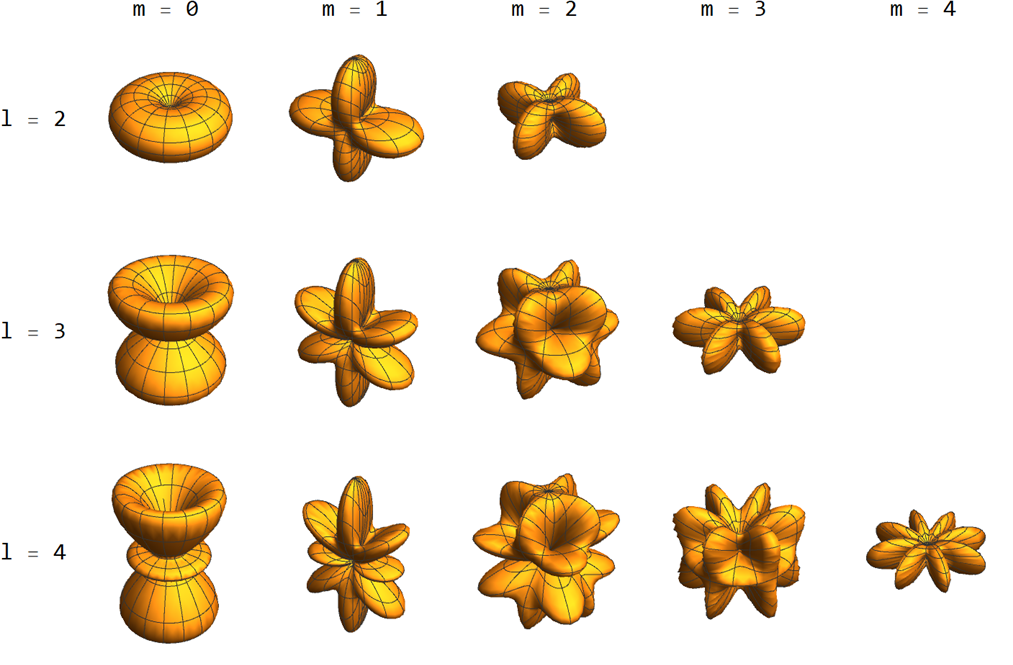
\includegraphics[width=0.8\textwidth]{angle-modes-odd-near}%
        \caption[]{Диаграммы направленности нечетных мод в ближней зоне, $\omega = 1$}%
        \label{fig:radpo-near}%
    \end{figure}

    \begin{figure}[!htb]%
        \centering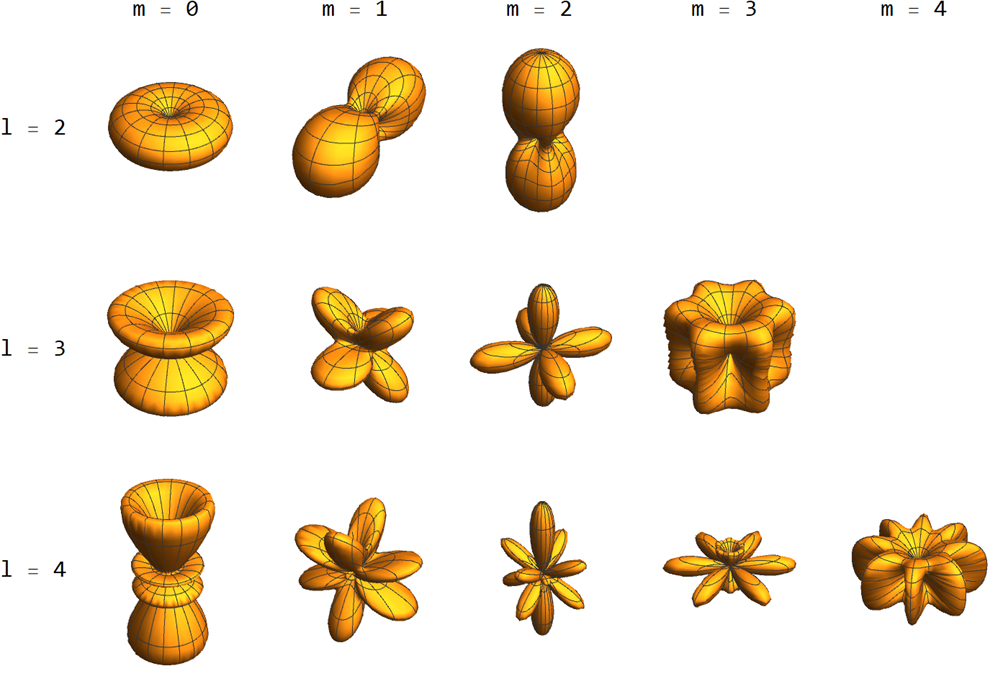
\includegraphics[width=0.8\textwidth]{angle-modes-odd-far}%
        \caption[]{Диаграммы направленности нечетных мод в дальней зоне, $\omega = 1$}%
        \label{fig:radpo-far}%
    \end{figure}

    Из \autoref{fig:radpo-near} и \autoref{fig:radpo-far} видно, что в ближней и дальней зоне диаграммы направленности могут различаться существенно. Трансформация картины в ближней зоне в картину в дальней зоне, не показанная здесь, также носит довольно интересный характер.

\subsection{Плотность и поток энергии нечетных мод}

    В отличие от углового распределения излучения (диаграммы направленности), средняя энергия и средний поток энергии более показательны, чем их мгновенные значения. Средние плотность и поток энергии различаются как в зависимости от $l$, так и в зависимости от $m$. Для принципиального изучения как всегда более интересны наиболее простые случаи, т.е. конфигурации с $m=0$.

    Энергия произвольной моды содержит как постоянную, так и переменную (убывающую на бесконечности как $r^{-2}$) составляющие.

    Поток энергии базовой моды всегда имеет нулевую компоненту $U^\varphi$, что упрощает его изучение. Компонента $U^\theta$ убывает на бесконечности как $r^{-3}$. Компонента $U^r$ имеет постоянную (не зависящую от $r$) составляющую, переменная составляющая же убывает как $r^{-2}$. При любом $l$ и любом $m$ лишь $U^r$ содержит постоянную составляющую: поток энергии на бесконечности может быть направлен лишь радиально от источника.

    На \autoref{fig:Ui-vec-odd} изображена векторная диаграмма потока энергии в ближней зоне для базовой моды. Хорошо наблюдается наличие зон реверсивного потока вблизи нуля, а также наличие стационарных точек потока, в которых он обращается в нуль. Присутствие реверсивной составляющей потока обеспечено наличием отрицательных областей у компонент потока энергии в ближней зоне. Количество стационарных точек определяется числом $l$.

    Ни средний поток, ни средняя плотность энергии не зависят от $\varphi$, что легко объяснимо видом этой зависимости ($\exp(i m \varphi)$). Однако компонента $U^\varphi$ при $ m \neq 0$ отлична от нуля и убывает на бесконечности также, как и переменная составляющая $U^r$, т.е. медленнее, чем $U^\theta$.

    \begin{figure}[!htb]%
        \centering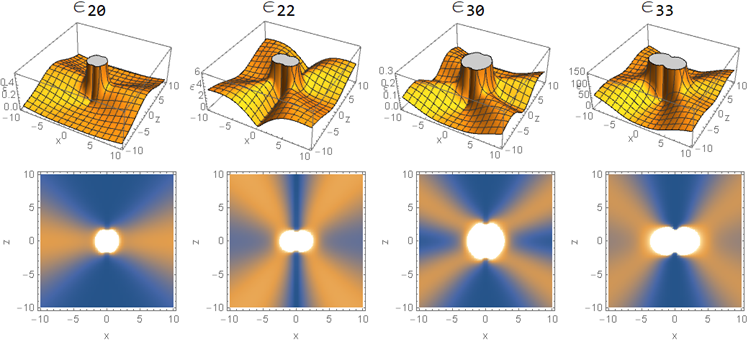
\includegraphics[width=0.8\textwidth]{energy-odd}%
        \caption[]{Плотность энергии излучения нечетных мод, $\omega = 1$}%
        \label{fig:eps-odd}%
    \end{figure}

    \begin{figure}[!htb]%
        \centering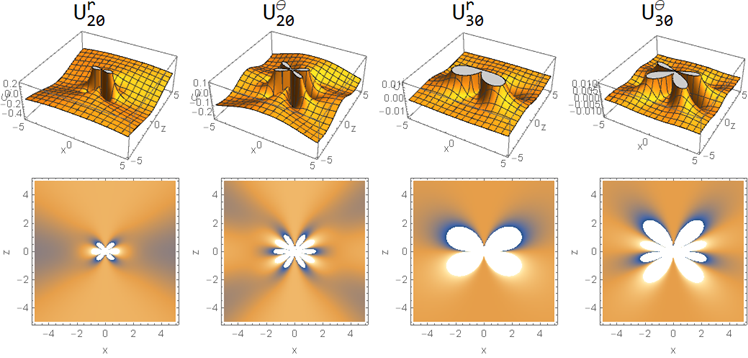
\includegraphics[width=0.8\textwidth]{pointing-odd}%
        \caption[]{Компоненты вектора потока энергии нечетных базовых мод, $\omega = 1$. Темно-синий цвет соответствует отрицательным областям}%
        \label{fig:Ui-odd}%
    \end{figure}

    \begin{figure}[!htb]%
        \centering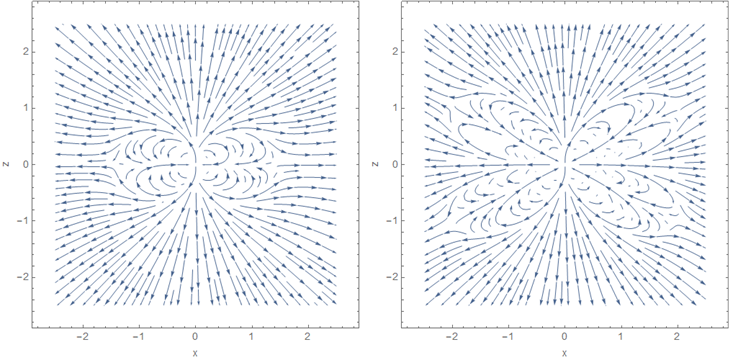
\includegraphics[width=0.8\textwidth]{pointing-vec-odd}%
        \caption[]{Векторные диаграммы потока энергии нечетных базовых мод ($l=2$ и $l=3$) в ближней зоне, $\omega = 1$. Стационарные точки (для правой полуплоскости): $\qty(\sqrt{2},\flatfrac{\pi}{2})$ для $l=2$ и $\qty(\sqrt{5},\acos(\pm\flatfrac{1}{\sqrt{5}}))$ для $l=3$}%
        \label{fig:Ui-vec-odd}%
    \end{figure}

\end{document}
